
\section{ISC Hadoop MapReduce}\label{sec:design}
This section describes the system co-design of our In-Storage Computing model and Hadoop MapReduce framework.


%\textcolor{red}{1. architecture, 2. execution time analysis (mapper, shuffle, reduce, etc), why offload mapper, biggest portion, 3. flow chart explanation. Challenge added: mapping HDFS to a local file. 4. ISC is not always good solution. io intensive is the best app. cpu intensive is not good. 5. one node, multi real cluster. 6 multinodes Pseudo distributed mode, 7. data transfer comparision in bus anlyzer, 7. fully distributed mode on a single machine}




\begin{figure}[htbp]
%\vspace{-5mm}
	\centering
		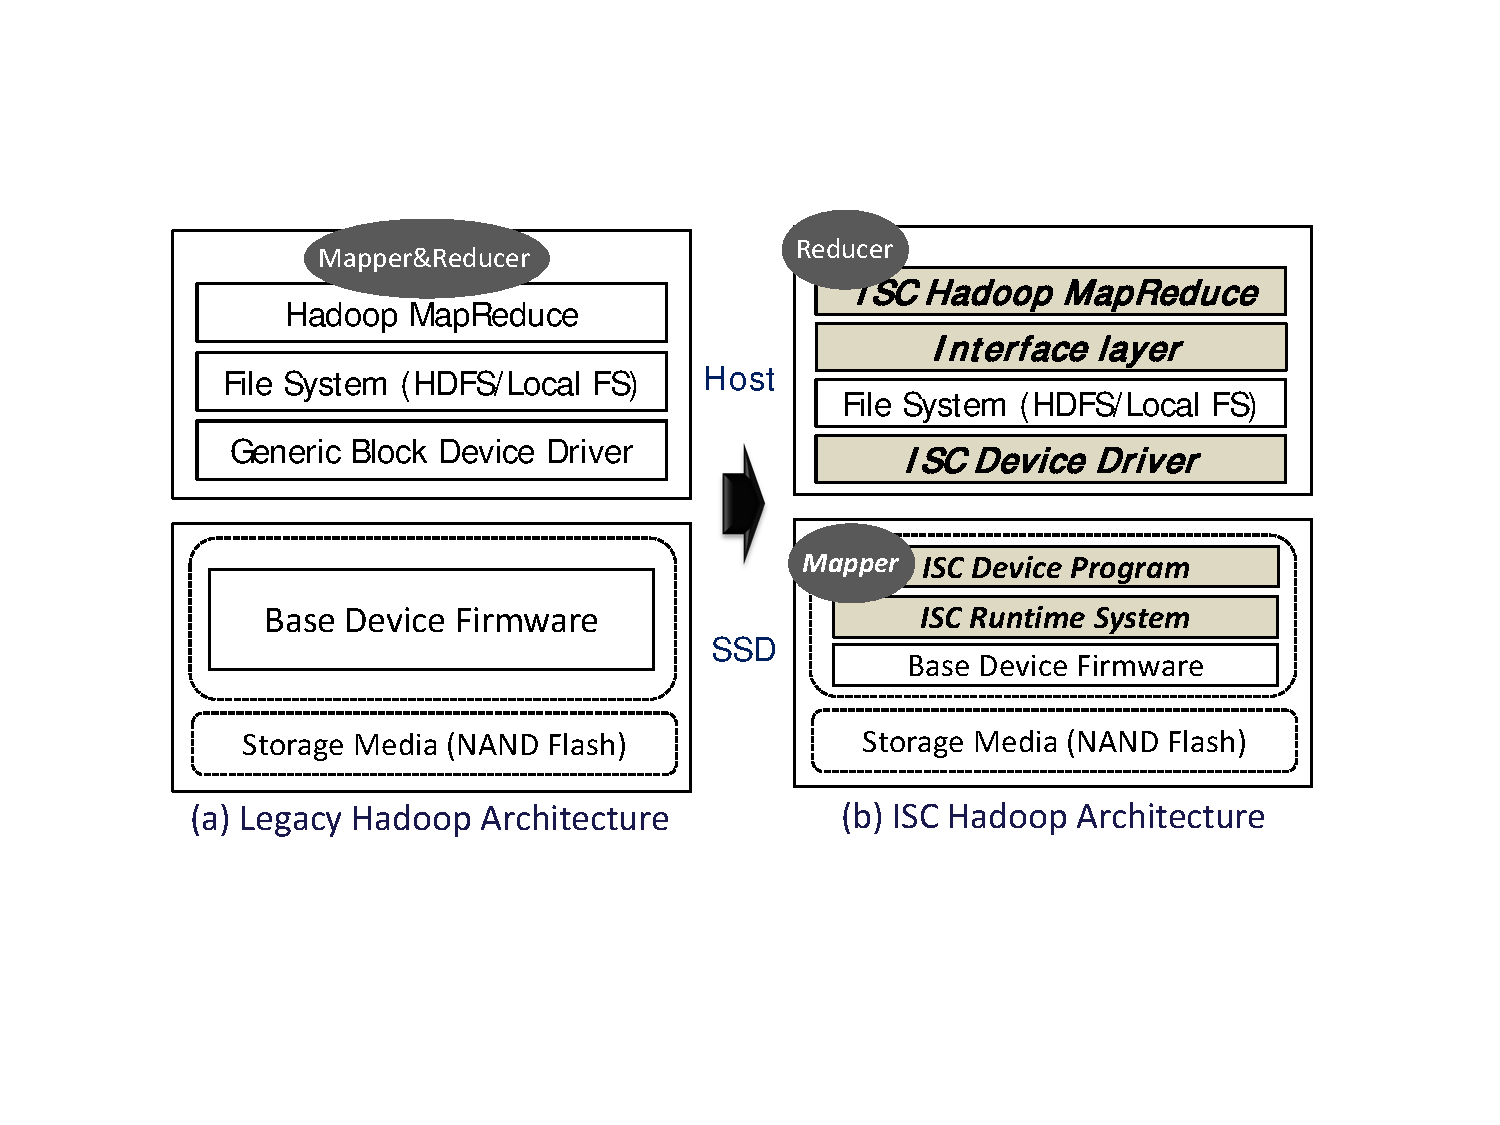
\includegraphics[width=1.0\columnwidth]{figures/ISC_Hadoop_architecture3.pdf}
	\caption{ISC Hadoop MapReduce architecture}
	\label{fig:ISC_Hadoop_arch}
\end{figure}


\subsection{System Architecture}\label{sec:designSpace}
Figure~\ref{fig:ISC_Hadoop_arch} shows an overall system architecture of our ISC Hadoop MapReduce framework. As explained, we offload the Mapper into an ISC device and implement the Mapper feature inside the real SSD firmware. Thus, a host Hadoop MapReduce system must be revised to collaborate with our ISC device thereby disabling Mapper features in the host system and implementing them inside SSD firmware (i.e., ISC device program). To support ISC functions, we also need to develop ISC engines (i.e., ISC Runtime System) on top of the existing base device firmware. The interface layer plays a role of an agent in communication between the host Hadoop MapReduce system and our ISC MapReduce system. We suggest this software component to resolve two major design issues: discrepancy in system interfaces and discrepancy in data representation between the host and the ISC devices (these issues will be addressed in the subsection~\ref{subsubsec:data_represent} and~\ref{subsubsec:system_interface} in detail.).
Alongside of a generic SCSI block device driver, we implement a special SCSI command to trigger ISC features inside the SSD (ISC Device Driver). We do not touch both HDFS and a local file system. So, our ISC Hadoop MapReduce system seamless supports all existing Hadoop features.   
%Moreover, to integrate our ISC Hadoop MapReduce model to the existing Hadoop MapReduce framework, we change Hadoop MapReduce components accordingly in the host for an ISC computing model, and develop an ISC device driver for the communication between the host system and our ISC device.

We first explore our work on a single Hadoop machine to verify our idea and concept, and then extend our design to Hadoop clusters of multiple nodes.


\begin{figure}[htbp]
%\vspace{-5mm}
	\centering
		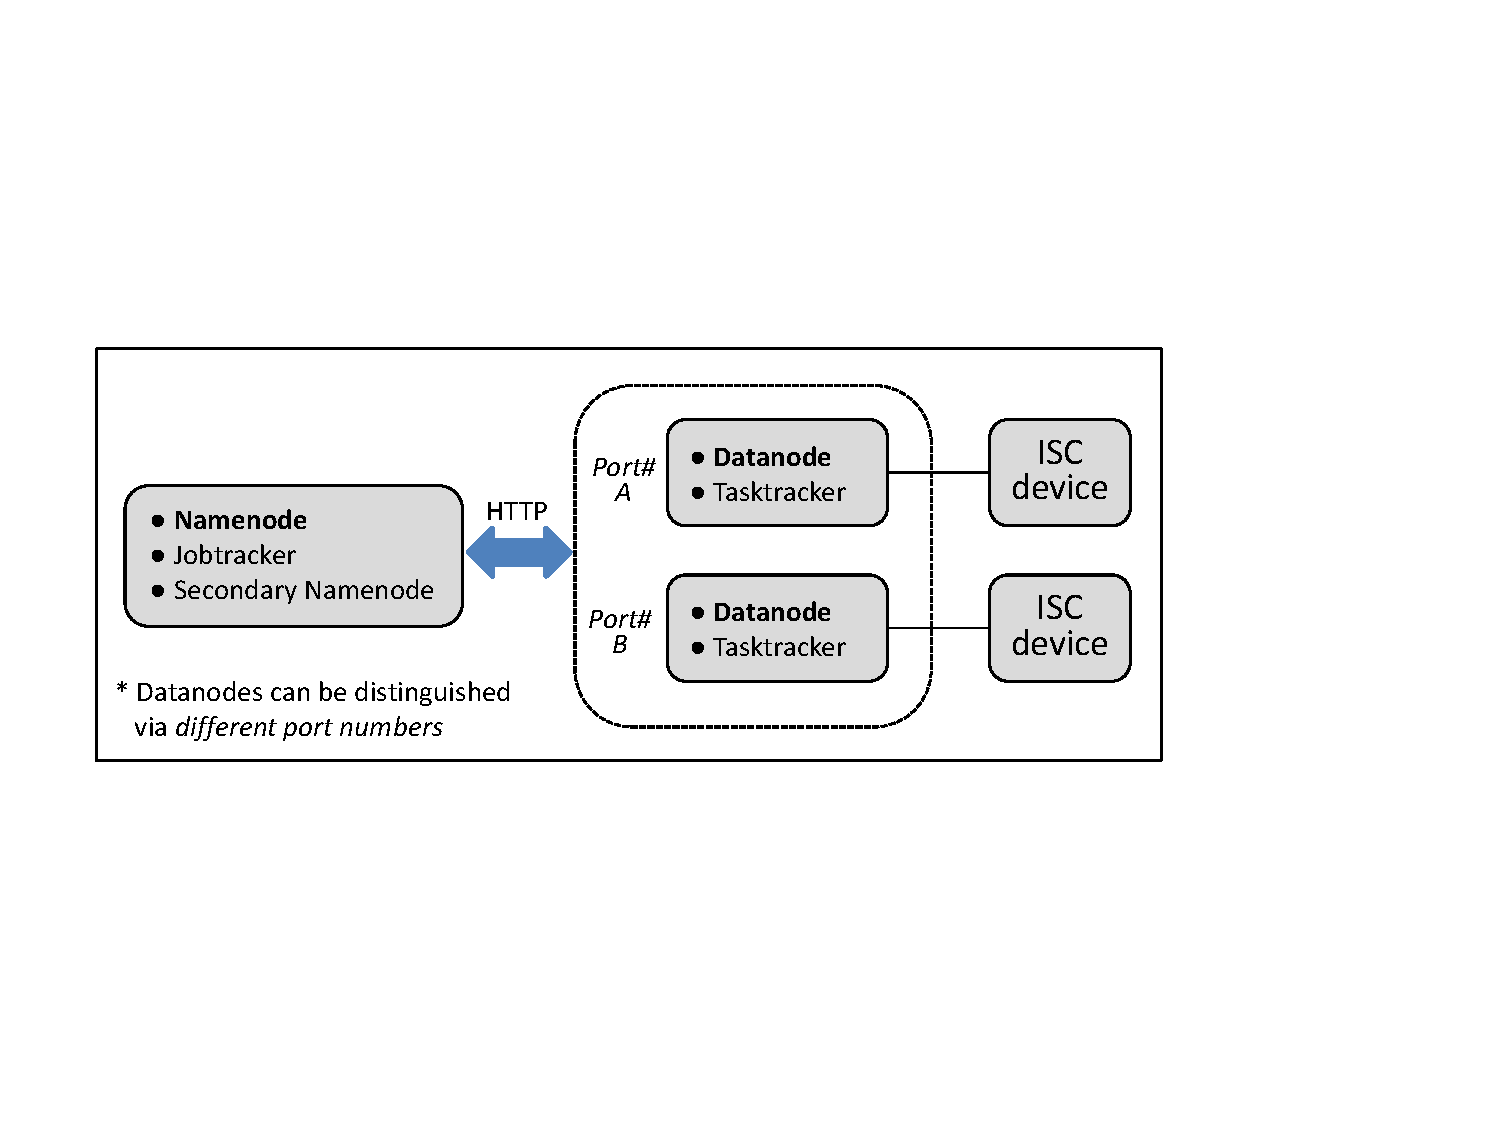
\includegraphics[width=1.0\columnwidth]{figures/Single_node_architecture.pdf}
	\caption{ISC Hadoop configuration on a single node: a fully distributed mode on a single machine}
	\label{fig:ISC_single_node_config}
\end{figure}

\subsubsection{A Single Node}\label{subsubsec:singlenode}
There are typically three ways to install and configure Hadoop: a local (standalone) mode, a pseudo distributed mode, and a fully distributed mode. In the standalone mode, all Hadoop components (i.e., namenode, jobtracker, datanode, tasktracker, secondary namenode) run in a single Java process (i.e., JVM instance) and this mode does not use HDFS. In the pseudo distributed mode, Hadoop runs all the components as separate Java processes and uses HDFS. This serves as a simulation for fully distributed Hadoop clusters but it runs \emph{a single instance of datanode on a single machine} only. The fully distributed mode runs on clusters of multiple machines with a master (plays namenode and job tracker. Optionally secondary namenode) and slaves (plays datanodes and tasktrackers) concept~\cite{MapReduce:Tutorial}. 

As described, basically it is impossible to run Hadoop in a fully distributed mode on a local machine (i.e., \emph{multiple instances of datanode on a single machine}). We, however, install and configure Hadoop in the fully distributed mode on a single node with a workaround, which is very efficient to initially verify our proposed ISC Hadoop MapReduce framework. Figure~\ref{fig:ISC_single_node_config} illustrates this Hadoop configuration on a single node. We configure separate Hadoop configuration files for each datanode instance. For HTTP communication with the namenode, we assign different port numbers for each datanode instance, wherein each datanode connects with our ISC device. Thus, each datanode can be distinguished via different port numbers for communication with the datanode\footnote{\small This configuration is based on Hadoop 0.20.205 and we found the assignment of virtual IPs to each datanode instance did not work for this workaround in this Hadoop version.}. This workaround mode represents the fully distributed Hadoop clusters on a single node.
 % and we found this performed very well (all the experiments of this configuration will be described in our experiment section in detail).



\subsubsection{Clusters: Multiple Nodes}\label{sec:multinodes}
The aforementioned single node configuration represents well the main features of the distributed Hadoop clusters on a local machine. Based on this observation, we extend our ISC Hadoop MapReduce framework to real Hadoop clusters. We set up the clusters of 5 nodes and separate a namenode from other datanodes (i.e., 1 namenode and 4 datanodes) to completely eliminate its performance overheads from the datanode. We initially start our study with one datanode and gradually increase the number of datanode to four on our clusters. Since we found meaningful and predictable performance results (that is, almost linear performance increase), we did not set up the bigger Hadoop clusters (please refer to our experiment results).


\begin{figure}[htbp]
%\vspace{-5mm}
	\centering
		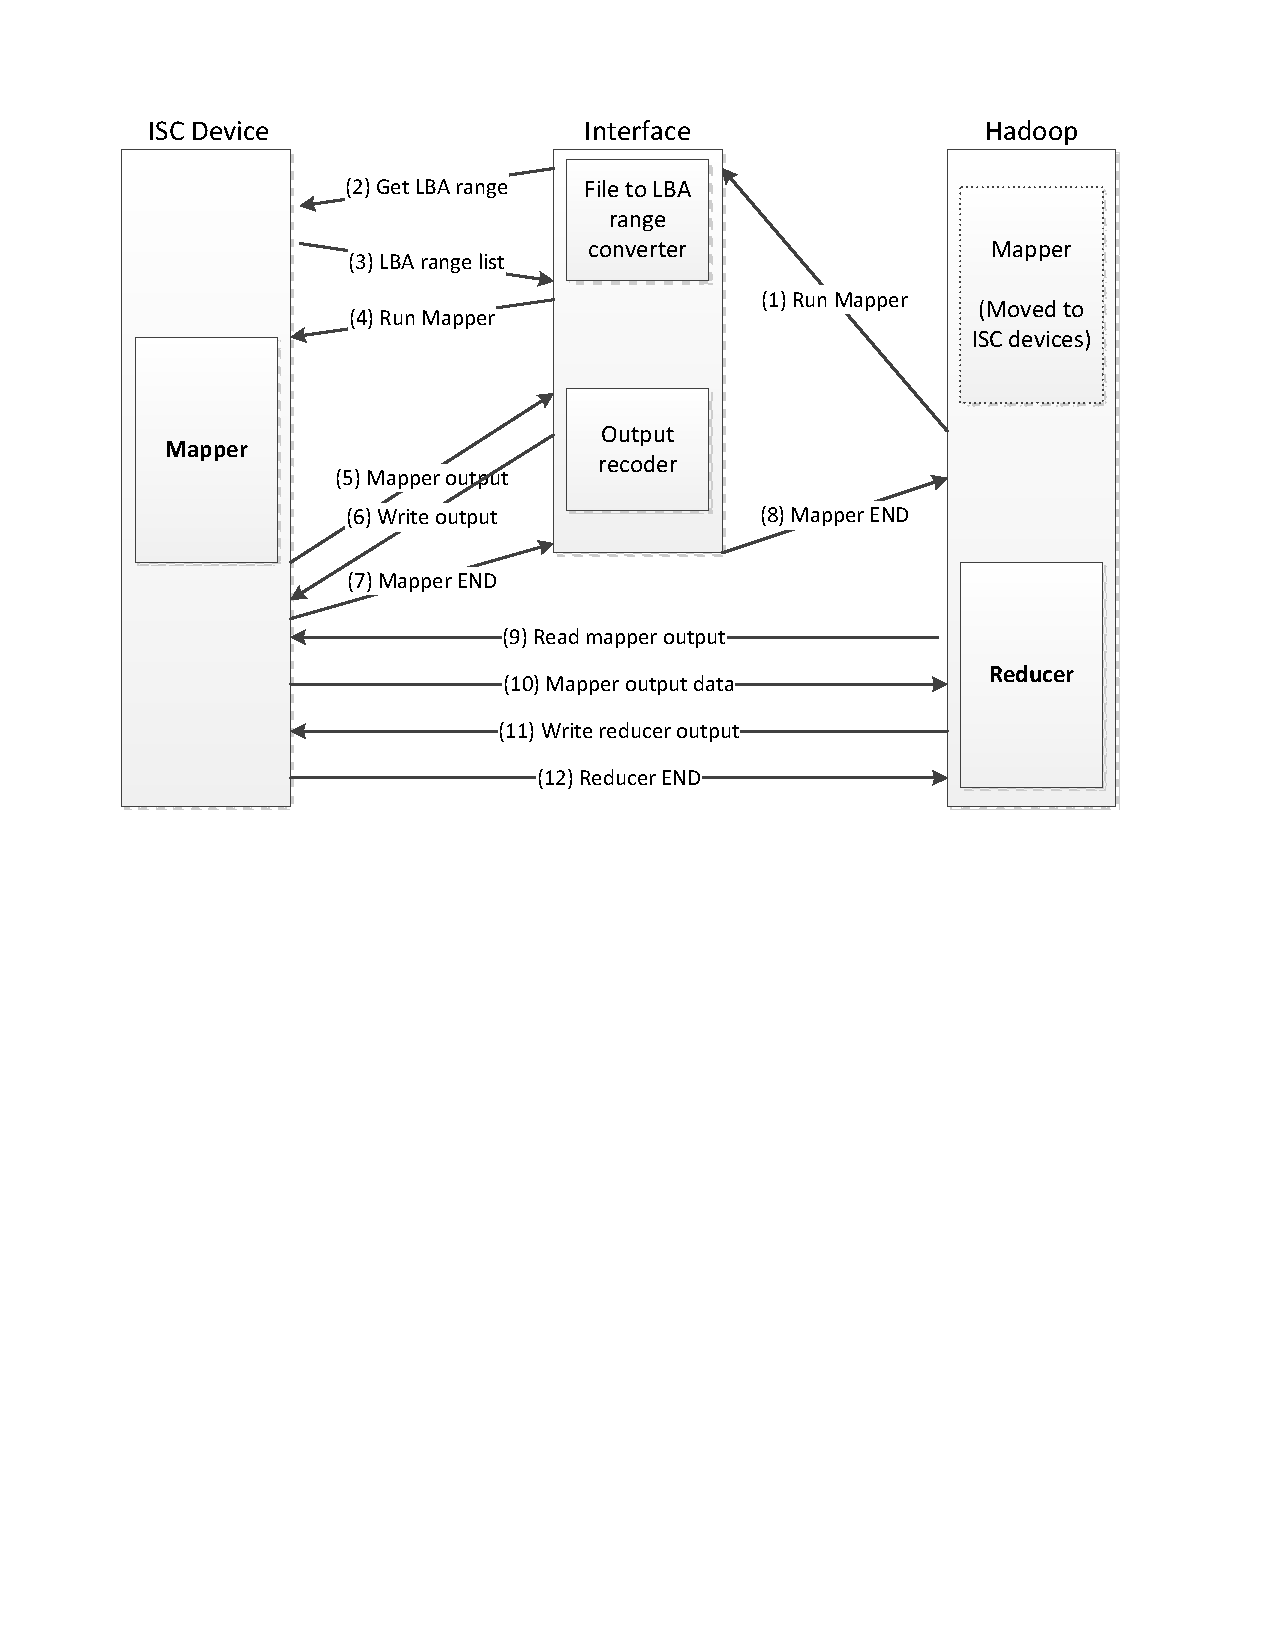
\includegraphics[width=0.98\columnwidth]{figures/ISC_Hadoop_Flowchart.pdf}
	\caption{ISC Hadoop MapReduce workflow}
	\label{fig:ISC_Hadoop_flow}
\end{figure}




\subsection{Workflow}\label{sec:workflow}
Figure~\ref{fig:ISC_Hadoop_flow} depicts our ISC Hadoop MapReduce workflow. Once a Hadoop application runs, our ISC Hadoop MapReduce framework does not directly run Mappers in the host system because they moved inside ISC devices. Instead, it first calls an interface component to communicate with ISC devices while delivering the input split data information (i.e., a file name of the input split) for ISC Map tasks. The interface runs its software component for converting each input split data (64MB) information to different data representation (i.e., LBA range information) for ISC devices. We found each input data of 64MB is generally split further into 2 or 3 smaller data chunks via an EXT4 file system. This means the software component in the interface (i.e., File to LBA range converter) delivers 2 or 3 LBA range lists to an ISC device for each Map task.
That is, the interface component calls Mapper inside the ISC device with these converted LBA range lists. After the Mapper receives all metadata information from the interface layer, it starts to execute a Map task. Once the Map task completes, the ISC devices return their Mapper outputs (i.e., intermediate results) to the interface layer to save them in the device (that is, the Mapper outputs are written with a local file system.). In fact, these Map output writing processes (Step 5 and 6) can be replaced with our new ISC API--PUT. Now, Reducers in the host can start to read the intermediate data as their input values and perform Reduce tasks. Finally all Map and Reduce tasks completes, our Hadoop system stores the final results with Hadoop Distributed File System (HDFS).



\subsection{Design Challenges}\label{sec:challenges}
This section addresses the challenging issues to design our ISC Hadoop MapReduce framework.

\subsubsection{Discrepancy in Data Representation}\label{subsubsec:data_represent}
To access data in a device, a host system can use file system information and so does the host Hadoop system by employing HDFS or local file systems such as EXT3/4. However, the device itself cannot rely on any file system information to access data inside its own device for ISC processing. This discrepancy in data representation between the host and the device causes an essential problem. This is the main reason the previous ISC work~\cite{SmartSSD:SIGMOD:2013,SmartSSDHadoop:MSST:2013} had no choice but to write their data to the raw device with 'dd' command by explicitly specifying their data locations (LBAs) from the beginning. This approach can temporarily evade this issue; but cannot resolve it. Consequently, it gives rise to other critical limitations on their systems. For instance, Kang et al. proposed a Hadoop MapReduce system leveraging ISC computation~\cite{SmartSSDHadoop:MSST:2013}. However, due to this challenging issue, their Hadoop system works only one local machine (i.e., no scalability) since it cannot support HDFS and local file systems. 
  
We fundamentally figure out this critical issue by developing a software component in the interface layer between the Hadoop system and ISC devices (please refer to the Figure~\ref{fig:ISC_Hadoop_flow}). This component is in charge of converting a file name into LBA range list information for the ISC device. Therefore, our proposed ISC Hadoop MapReduce system can seamlessly support the existing Hadoop features. For this, we first get a local file system information of each data split (64MB) from HDFS and convert it to LBA range lists. Then we deliver this information to ISC devices for Map tasks.


\subsubsection{Discrepancy in System Interfaces}\label{subsubsec:system_interface}
System interfaces between Hadoop framework in the host system and ISC device can be different. That is to say, Hadoop MapReduce framework in the host adopts Java programming language, while our SSD firmware for ISC processing uses C/C++ language. As a result, the host Hadoop system cannot directly communicate with ISC devices. To resolve this issue, we can think of two options: (1) running OS inside ISC devices and (2) adopting an interface layer. If an OS runs inside ISC device, it can also simply run JVM on top of the OS. This solution looks like very intuitive and may be able to eliminate our aforementioned challenge (i.e., discrepancy in data representation). However, this approach requires to consume extra ISC computing resources such as CPU and DRAM inside the device. Thus, unless the ISC device is a very specialized device with powerful computing resources, the first option will not be a good choice. 

As a matter of fact, since our ISC device is a typical commodity SSD without enough computing resources, we choose the second option. We, instead, put another interface layer between the Hadoop system and ISC devices by adopting Java Native Interface (JNI). Aside from the programming system interface between them, this interface layer plays two important roles in our ISC Hadoop System--first, as mentioned above, converting a file name to LBA range information, and second, writing the output data (i.e., intermediate data) of ISC Map tasks. For this, the host Hadoop system needs to deliver metadata information including an input split file name and an output file name of the intermediate data. The overhead of this extra interface layer is almost ignorable.


\begin{figure}[htbp]
%\vspace{-5mm}
	\centering
		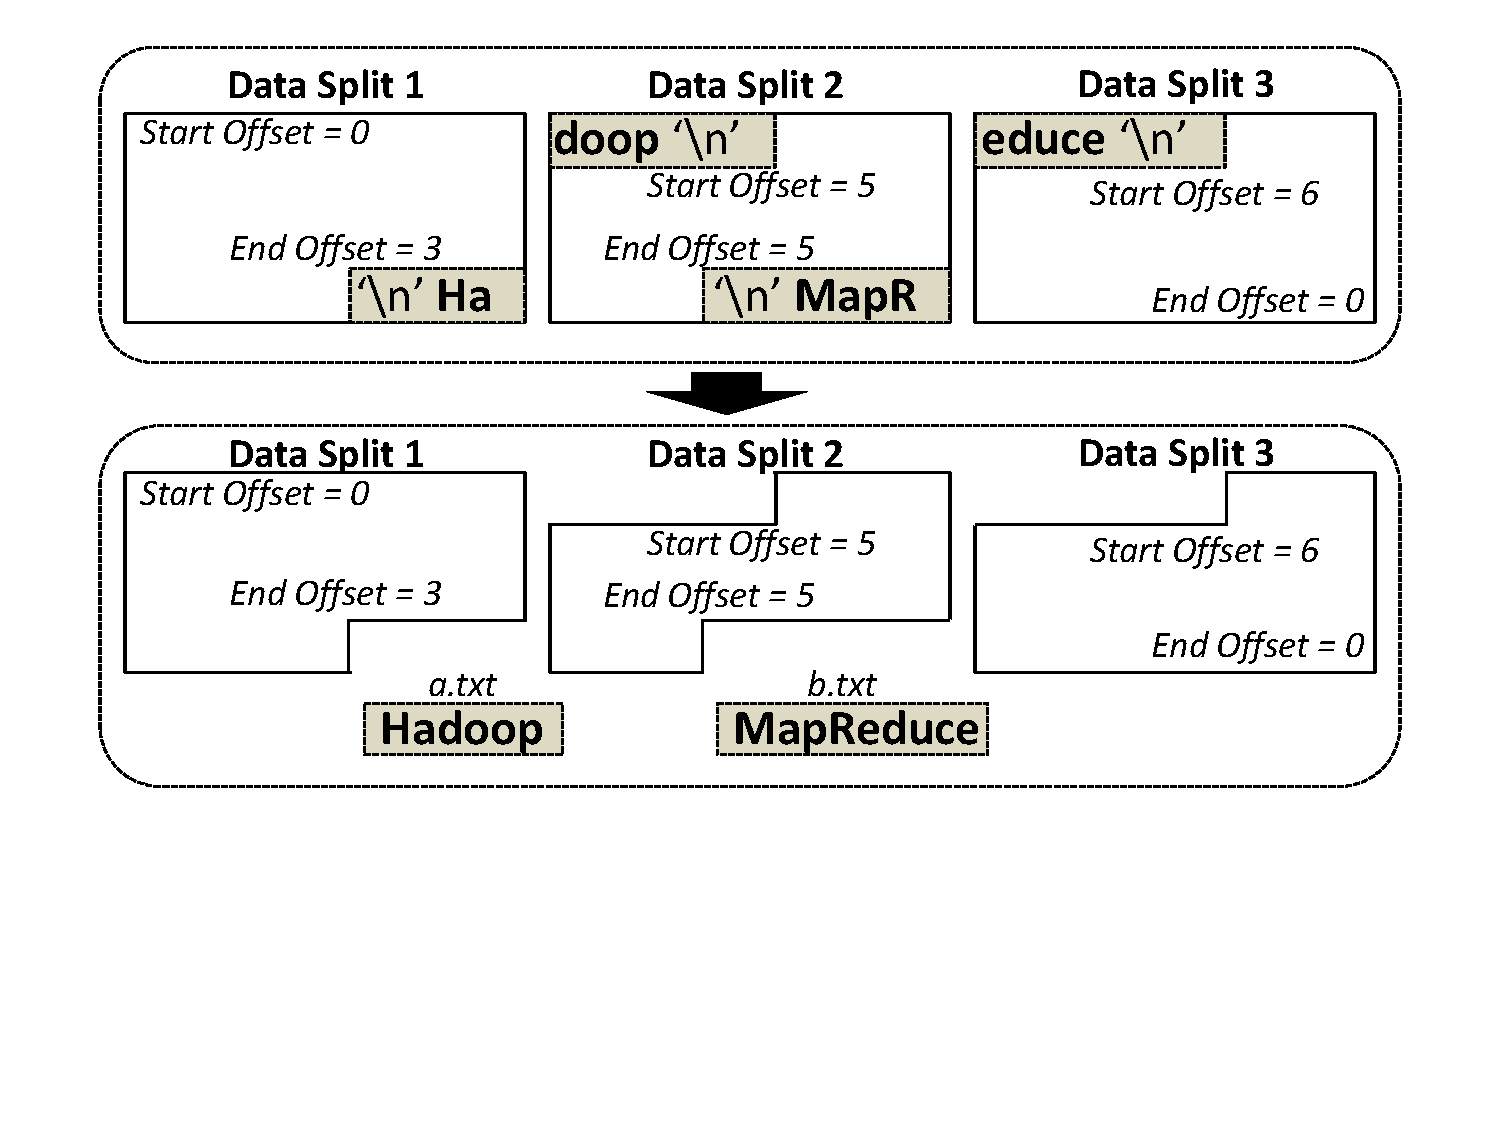
\includegraphics[width=1.0\columnwidth]{figures/Data_split_example2.pdf}
	\caption{A data split example}
	\label{fig:data_split_example}
\end{figure}

\subsubsection{Data Split}\label{subsubsec:data_split}
Hadoop Distributed File System (HDFS) splits large input data into a chunk of 64MB by default~\cite{TomWhite:HadoopDefinitiveGuide:2012}. This input split process raises another critical problem in ISC Hadoop system: data split. Figure~\ref{fig:data_split_example} illustrates this issue. Assuming a word data 'Hadoop' is stored in the large input data, HDFS may split the word 'Hadoop' into 'Ha' in one file of 64MB (i.e., Data Split 1) and 'doop' in another file of 64MB (i.e., Data Split 2) if the word inadvertently lies in the input split boundary. This does not causes any issue in a typical Hadoop system because HDFS in the host Hadoop system loads all input split data in the main memory and processes them in a streaming data access manner. However, since ISC Hadoop MapReduce framework basically does not move input data from devices to the host memory, this data split issue can cause a critical problem in the ISC Hadoop system. If the ISC device is equipped with such a capability that they can directly connect/communicate with each other like Ethernet-connected drives (e.g., Seagate's Kinetic HDD or HGST's Ethernet Drive~\cite{KineticHDD:Seagate:2014,EthernetDrive:HGST:2014}), we may be able to solve this issue with a naive way, but unfortunately, our ISC drive is not equipped with such a communication interface.

To resolve this, our ISC Hadoop system consults the host Hadoop system. If the host Hadoop system detects a split data\footnote{\small Host Hadoop system originally has a simple algorithm for this data split detection.}, it stores the split data (both Hadoop and MapReduce in the example) as a separate file respectively with a local file system. Then it converts the file name to LBA information by using the aforementioned software component and delivers the LBA information to the ISC device via the interface layer. To avoid inaccurate (i.e., duplicated) computation of that part inside ISC device, the host system provides the ISC device with another metadata information (that is, Start Offset and End Offset) for each data split. These offsets can be thought of as data lengths of each part including a delimiter, where the delimiter can be a carriage return, space, or tab, depending on the Hadoop applications. With the help of this metadata information, ISC Mapper can simply ignore processing all the data within the offset boundary in each data split chunk of 64MB.


%To resolve this, our ISC Hadoop system consults the host Hadoop system. If the host Hadoop system detects a split data\footnote{\small Host Hadoop system originally has a simple algorithm for this data split detection.}, it stores the split data as a separate file with a new file name. Then it converts the file name to LBA information and delivers the LBA information to the ISC device. To avoid inaccurate (i.e., overlapped) computation of that part inside ISC device, the host system should provide another metadata information regarding this overlapped part which should not be processed by ISC Mapper. For this, the host system provides its offset information to ISC device as metadata and the ISC device simply ignore all the data with the offset in the file.


\subsubsection{Feature Offloading}\label{subsubsec:feature_offloading}
%As discussed in the Section~\ref{sec:ISC_background} and previous work~\cite{SmartSSD:SIGMOD:2013,SmartSSDHadoop:MSST:2013}, our ISC model can be best utilized by the applications with the following characteristics: (1) I/O intensive (not heavily CPU intensive), (2) less data access per data page (i.e., 8KB flash memory page), and (3) a smaller amount of output data after data processing. I/O intensive applications can leverage a high internal bandwidth of SSDs and the less data access per data page is closely related to the low DRAM performance inside SSDs. If the ratio of the amount of data after processing vs. that of before processing is close to 1, these applications discard ISC performance gain thereby transferring the large final output data to a host system. Based on these observations, a database application best fits for those requirements~\cite{SmartSSD:SIGMOD:2013}. However, in this work, we explore another application for our ISC model: Hadoop MapReduce. 


The data precessing of Hadoop MapReduce framework is composed of Map and Reduce. Unlike a Map task that does not have any dependency among other tasks for its execution, a Reduce task is inherently dependent on other Map task executions. That is, a Reducer is required to collect output results of other Map tasks in its shuffle phase before a Reduce task starts. However, as we mentioned in the previous subsection~\ref{subsubsec:data_split} (Data Split), our ISC device is not equipped with such a communication capability, a host system should be in charge of collecting the intermediate data from each Mapper. Moreover, the host should redistribute the collected data to each ISC device for the Reduce execution. Not only can these processes incur unnecessary data movement traffic, but also can the ISC devices be overwhelmed by the overburden because typically an ISC device has very limited resources and both Mapper and Reducer, in general, are executed concurrently.

Many Hadoop MapReduce applications (not necessarily, but mostly) produce small amount of intermediate data after a Map task processes original big data. In addition, the Reduce task is subdivided into three major phases such as copy, sort, and reduce. Unlike a Map task, the Reduce task generally does not significantly lessen the data size of its output result after Reduce processing. This is not favorable to ISC framework~\cite{SmartSSD:SIGMOD:2013}. The sort can give rise to another unfavorable issue. Assuming a data size is bigger than an available DRAM space in an ISC device, it may have to issue tremendous NAND flash Write operations to store intermediate results, which has a critical impact on the life endurance of NAND flash memory~\cite{SSDDesignTradeOff:ATC:2008,IPL:SIGMOD:2007,HotData:MSST:2011,HotDataTrap:ACR:2013}. 

Based on these observations, we move Mapper to ISC devices, not Reducer, in the Hadoop MapReduce framework.



%Based on these observations, we move Mapper to ISC devices, not Reducer, in the Hadoop MapReduce framework. In general, many Hadoop MapReduce applications produce small amount of intermediate data after Map tasks process original big data. In addition, the Reduce task is subdivided into three major phases such as copy, sort, and reduce. Unlike a Map task, the Reduce task generally does not significantly lessen the data size of its output result after Reduce processing. This is not favorable to ISC framework~\cite{SmartSSD:SIGMOD:2013}. Moreover, the sort phase may require tremendous Write operations to store intermediate results, which has a critical impact on the life endurance of NAND flash memory~\cite{SSDDesignTradeOff:ATC:2008,IPL:SIGMOD:2007,HotData:MSST:2011,HotDataTrap:ACR:2013}. 



\subsection{Hadoop Applications}\label{sec:application}

As discussed in the Section~\ref{sec:ISC_background} and previous work~\cite{SmartSSD:SIGMOD:2013,SmartSSDHadoop:MSST:2013}, our ISC model can be best utilized by the applications with the following characteristics: (1) I/O intensive (not heavily CPU intensive), (2) less data access per data page (i.e., 8KB flash memory page), and (3) a smaller amount of output data after data processing. I/O intensive applications can leverage a high internal bandwidth of SSDs and the less data access per data page is closely related to the low DRAM performance inside SSDs. If the ratio of the amount of data after processing vs. that of before processing is close to 1, these applications discard ISC performance gain thereby transferring the large final output data to a host system. Based on these observations, a database application best fits for those requirements~\cite{SmartSSD:SIGMOD:2013}. In this work, we explore another application for our ISC model: Hadoop MapReduce. We can find many Hadoop applications with I/O intensive and generally they produce a smaller amount of final outputs after processing input data. 
However, unfortunately, Hadoop applications cannot meet the second characteristics (less data access per data page) since they have to read every single byte of all data to process them.

Admittedly, all Hadoop applications cannot benefit from our ISC Hadoop MapReduce framework. We now explore various Hadoop applications to choose an appropriate application for our experiment and discuss the rationale of the choice. 

For this Hadoop application study, we refer to Purdue MapReduce (PUMA) Benchmarks Suite~\cite{PUMA:Purdue:2012}. PUMA benchmark suite presents a broad range of Hadoop MapReduce applications (i.e., a total of 13 applications) exhibiting various application characteristics. We run PUMA benchmark on our Hadoop machine and analyze each application for our study. After the investigation, interestingly, we found many of the applications (7 out of 13 including wordcount) can be classified into a wordcount-like application. That is to say, (1) a processed data size is a lot smaller than an original data size, (2) average per-Mapper execution time is a lot longer than the average per-Reducer execution time (i.e., Mapper intensive), (3) their final results produce counting-related values, and (4) generally CPU intensive but not highly CPU intensive computation.

For the rest of applications, particularly, Terasort can be identified as a worst Hadoop MapReduce application for our ISC framework. Sorting applications including Terasort never reduce their processed data size, which is a very unfavorable characteristic to ISC framework~\cite{SmartSSD:SIGMOD:2013}. More critically, due to a limited DRAM resource inside our ISC devices, Terasort should generate an enormous number of flash write operations to temporarily store its intermediate data. This can critically impact NAND flash lifetime.
K-means clustering is another unfavorable MapReduce application for our ISC framework because an amount of transferring data is never reduced and instead it is even increased with extra information via many iterations. Moreover, relatively high CPU computation is required to calculate the cosine-vector similarity of a given data with all the centroids.

Based on our study, we choose Hadoop wordcount as our ISC application. As we mentioned above, this wordcount is a very representative application and many other benchmark programs (term-vector, inverted-index, histogram-movies, histogram-ratings, sequence-count, ranked-inverted-index, etc) retain a very similar characteristics to the wordcount application. Thus, we expect very similar results and implications to run other applications of them. Actually, several of them use the same input data as wordcount and exhibit even almost the same execution time as the wordcount based on our experiments. We could choose other ISC-favorable applications instead of the wordcount. However, its representativeness led us to go with it. 
The main goal of this work is not to run various Hadoop applications, but to verify our ISC Hadoop MapReduce framework and to explore its opportunities and challenges. Therefore, we leave implementing/running various applications including even ISC-unfavorable ones on top of our ISC framework as our future work.




%\textbf{Step S4: Execute list operations}. The main reason of loading inverted lists to the host memory is to efficiently execute list operations such as intersection. Thus, both steps S4 and S3 should be offloaded to Smart SSDs. This raises another question: what operation(s) could potentially benefit from Smart SSDs. In Lucene, there are three basic operations commonly used: list \textsf{intersection}, \textsf{union}, and \textsf{difference}. They are also widely adopted in many commercial search engines (e.g., Google advanced search\footnote{\small\url{http://www.google.com/advanced_search}}). We investigate each operation and set up a simple principle that the output size should be smaller than its input size. Otherwise, Smart SSDs cannot save any data movement. Let $A$ and $B$ be two inverted lists, and we assume $A$ is shorter than $B$ to capture the real case of skewed lists.
%\begin{itemize}%[noitemsep, topsep=2pt]
 % \item \textsf{Intersection}: The result size of the intersection is usually much smaller compared to each inverted list, i.e., $|A\cap B| \ll |A| + |B|$. E.g., in Bing search, for 76\% of the queries, the intersection result size is two orders of magnitude smaller than the shortest inverted list involved~\cite{Ding2011}. Similar results are observed in our real dataset. Thus, executing intersection inside SSDs may be a smart choice as it can save a lot of host I/O interface bandwidth.

 % \item \textsf{Union}: The union result size can be similar to the total size of the inverted lists. That is because $|A\cup B| = |A| + |B| - |A\cap B|$, while typically $|A\cap B| \ll |A| + |B|$, then $|A\cup B| \approx |A| + |B|$. Unless $|A\cap B|$ is similar to $|A| + |B|$. An extreme case is $A = B$, then $|A\cup B| = |A| = |B|$, meaning that we can save 50\% of data transfer. However, in general, it is not cost-effective to offload \textsf{union} to Smart SSDs.

 % \item \textsf{Difference}: It is used to find all the documents in one list but not in the other list. Since this operation is ordering-sensitive, we consider two cases: $(A - B)$ and $(B - A)$. For the former case, $|A - B| = |A| - |A\cap B| < |A| \ll |A| + |B|$. That is, sending the results of $(A - B)$ saves a lot of data transfer if executed in Smart SSDs. On the other hand, the latter case may not save much data transfer because $|B - A| = |B| - |A\cap B| \approx |B| \approx |B| + |A|$. Consequently, we still consider the \textsf{difference} as a possible candidate for query offloading.
%\end{itemize}

%\textbf{Step S5: Compute similarity and rank}. After the aforementioned list operations are completed, we can get a list of qualified documents\footnote{\small Lucene assumes the results are small enough to fit into main memory, thus, no any I/O involved.}. %Lucene assumes the results are small enough to fit into main memory.
%This step applies a ranking model to the qualified documents in order to determine the similarities between the query and these documents. This is because users are more interested in the most relevant documents. This step is CPU-intensive so that it may not be a good candidate to offload to Smart SSDs. However, it is beneficial when the result size is very large because after step S5, only the top ranked results are returned. This can save a lot of I/Os. From the design point of view, we can consider two options: (1) do not offload step S5. In this case, step S5 is executed at the host side; (2) offload this step. In this case, step S5 is executed by Smart SSDs.


%\begin{table}[htbp]\small
%\centering
%\begin{tabular}{l|c|c}\hline\hline
%&Non-Ranked & Ranked \\\hline
%\textsf{Intersection} & \ding{51} & \ding{51} \\\hline
%\textsf{Union} &\ding{55}  & \ding{51}\\\hline
%\textsf{Difference} & \ding{51}& \ding{51}\\\hline\hline
%\end{tabular}
%\caption{Design space}\label{tab:designSpace}
%\end{table}
